%%%%%%%%%%%%%%%%%%%%%%%%%%%%%%%%%%%%%%%%%
% Thin Sectioned Essay
% LaTeX Template
% Version 1.0 (3/8/13)
%
% This template has been downloaded from:
% http://www.LaTeXTemplates.com
%
% Original Author:
% Nicolas Diaz (nsdiaz@uc.cl) with extensive modifications by:
% Vel (vel@latextemplates.com)
%
% License:
% CC BY-NC-SA 3.0 (http://creativecommons.org/licenses/by-nc-sa/3.0/)
%
%%%%%%%%%%%%%%%%%%%%%%%%%%%%%%%%%%%%%%%%%

%----------------------------------------------------------------------------------------
%	PACKAGES AND OTHER DOCUMENT CONFIGURATIONS
%----------------------------------------------------------------------------------------

\documentclass[a4paper, 12pt]{article} % Font size (can be 10pt, 11pt or 12pt) and paper size (remove a4paper for US letter paper)

\usepackage[protrusion=true,expansion=true]{microtype} % Better typography
\usepackage{graphicx} % Required for including pictures
\usepackage[utf8]{inputenc}
\usepackage[margin=1.0in]{geometry}
\usepackage{url}
\usepackage{fancyhdr}
\usepackage{amsmath}
\usepackage{setspace}
\usepackage{enumitem}
\usepackage{float}
\setlength\parindent{0pt} % Removes all indentation from paragraphs

\usepackage[T1]{fontenc} % Required for accented characters
\usepackage{times} % Use the Palatino font

\usepackage{listings}
\usepackage{color}
\lstset{mathescape}

\definecolor{dkgreen}{rgb}{0,0.6,0}
\definecolor{gray}{rgb}{0.5,0.5,0.5}
\definecolor{mauve}{rgb}{0.58,0,0.82}

\lstset{frame=tb,
   language=c++,
   aboveskip=3mm,
   belowskip=3mm,
   showstringspaces=false,
   columns=flexible,
   basicstyle={\small\ttfamily},
   numbers=none,
   numberstyle=\tiny\color{gray},
   keywordstyle=\color{blue},
   commentstyle=\color{dkgreen},
   stringstyle=\color{mauve},
   breaklines=true,
   breakatwhitespace=true
   tabsize=3
}
\linespread{1.00} % Change line spacing here, Palatino benefits from a slight increase by default

\makeatletter
\renewcommand{\@listI}{\itemsep=0pt} % Reduce the space between items in the itemize and enumerate environments and the bibliography
\newcommand\tab[1][1cm]{\hspace*{#1}}
\renewcommand\abstractname{Résumé}
\renewcommand\refname{Références}
\renewcommand\contentsname{Table des matières}
\renewcommand{\maketitle}{ % Customize the title - do not edit title and author name here, see the TITLE block below
\begin{center} % Right align

\vspace*{25pt} % Some vertical space between the title and author name
{\LARGE\@title} % Increase the font size of the title

\vspace{125pt} % Some vertical space between the title and author name

{\large\@author} % Author name

\vspace{125pt} % Some vertical space between the author block and abstract
Dans le cadre du cours
\\INF8225 - Techniques probabilistes et d'apprentissage
\vspace{125pt} % Some vertical space between the author block and abstract
\\\@date % Date
\vspace{125pt} % Some vertical space between the author block and abstract

\end{center}
}

%----------------------------------------------------------------------------------------
%	TITLE
%----------------------------------------------------------------------------------------

\title{TP3: } 
\author{\textsc{Guillaume Arruda 1635805} % Author
\vspace{10pt}
\\{\textit{École polytechnique de Montréal}}} % Institution

\date{19 Février 2016} % Date

%----------------------------------------------------------------------------------------

\begin{document}

\thispagestyle{empty}
\clearpage\maketitle % Print the title section
\pagebreak[4]
%----------------------------------------------------------------------------------------
%	En tête et pieds de page 
%----------------------------------------------------------------------------------------

\setlength{\headheight}{15.0pt}
\pagestyle{fancy}
\fancyhead[L]{INF8225}
\fancyhead[C]{}
\fancyhead[R]{TP3}
\fancyfoot[C]{\textbf{page \thepage}}

%----------------------------------------------------------------------------------------
%	ESSAY BODY
%----------------------------------------------------------------------------------------
\section*{Partie 1: Pseudocode}
Avec $\theta$ = W + b
pw\_linear(x) =\\
\tab    si x >= 0 \\
\tab\tab    retourne x \\
\tab	sinon \\
\tab\tab	retourne a * x \\

pw\_linear'(x) =\\
\tab	si x >= 0 \\
\tab\tab		retourne 1 \\
\tab	sinon \\
\tab\tab	retourne a \\
\\
softmax(x) = \\
\tab	retourne $\frac{exp(x)}{\sum{(exp(x_k))}}$ \\

Feedfoward(X) = \\
\tab	$activation_{0}$ = X + Colonne de 1 \\
\tab	Pour chaque couche cachée c \\
\tab\tab	pré-$activation_{c} = \theta_c * activation_{(c-1)}$ \\
\tab\tab	$activation_{c}$ = pw\_linear(pré-$activation_{c}$) + Colonne de 1 \\
\tab	$activation_{Finale}$ = softmax($\theta_{f} * activation_{c}$) \\

Backpropagate(X,Y) = \\
\tab	$delta_{final}$ = -(Y - $activation_{Finale}$) \\
\tab	pour chaque couche cachée c à partir de la fin \\
\tab\tab	D = pw\_linear'($pré-activation_{c}$) \\
\tab\tab	$delta_{c}$ = D .* $\theta_{(c+1)}$ * $delta_{(c+1)}$ \\ 
		
Update() = \\
\tab	pour chaque couche c \\
\tab\tab	$\theta_{c}$ = $\theta_{c}$ - tauxDapprentissage .* ($delta_{c}$ * $entrée_{c}$)\\

LossFunction(Y) = \\
\tab	retourne - ($\sum{Y .* log(activation_{Finale}}$)) \\

TrainNetwork(X,Y, Xvalid, Yvalid) = \\
\tab Tant que !converged    \\
\tab\tab    mbXs, mbYs = creer\_mini\_batch(X,Y)    \\
\tab\tab    pour chaque mbX, mbY dans mbXs, mbYs    \\
\tab\tab\tab    Feedfoward(mbX) \\
\tab\tab\tab    BackPropagate(mbX,mbY)  \\
\tab\tab\tab    Update()    \\
\tab\tab    Feedfoward(Xvalid)  \\
\tab\tab    loss = LossFunction(Yvalid) \\
\tab\tab    precision = calcul\_precision(YValid)    \\
\tab\tab    converged = loss > dernier\_lost

\section*{Partie 2: Résultats}
La première partie des expériences a permis de déterminer le nombre de neurone optimale dans le réseau à une couche
et à deux couches. Toutefois, il est rapidement devenu apparent que le nombre de neurone passé un certain point
a un effet marginale sur la performance du réseau, mais un effet significatif sur la performance.

\begin{table}[H]
\centering
\caption{Performance du réseau de neurone à une couche en fonction du nombre de neurone}
    \begin{tabular}{|l|c|c|c|}
        \hline
    	nombre de neurones & précision(\%) & perte moyenne & nombre d'itérations\\
    	\hline
    	800	    &	97.99    & 70.57 & 33\\
    	\hline
    	500		&	97.94	& 70.11 & 33\\
    	\hline
    	300		&	97.85	& 71.92 & 37\\ 
    	\hline
	    100		&	97.62	& 78.41 & 30\\
    	\hline
    \end{tabular}
\end{table}

\begin{table}[H]
\centering
\caption{Performance du réseau de neurone à deux couches en fonction du nombre de neurone}
\begin{tabular}{|l|c|c|c|}
	\hline
	nombre de neurones & précision(\%) & perte moyenne & nombre d'itérations\\
	\hline
	800,500	&	97.97	& 73.59  & 13\\
	\hline
	500,300	&	97.88	& 74.51  & 13\\
	\hline
	300,100	&	97.79	& 82.04  & 12\\
	\hline
	100,10	&	97.11	& 105.69 & 11\\
	\hline
\end{tabular}
\end{table}


Pour la création des courbes d'apprentissages suivantes, un réseau à une couche de 500 neurones a été utilisé et un réseau de deux couches de 500, 300 neurones a été utilisé.

\begin{figure}[H]
    \label{lossfunction}
    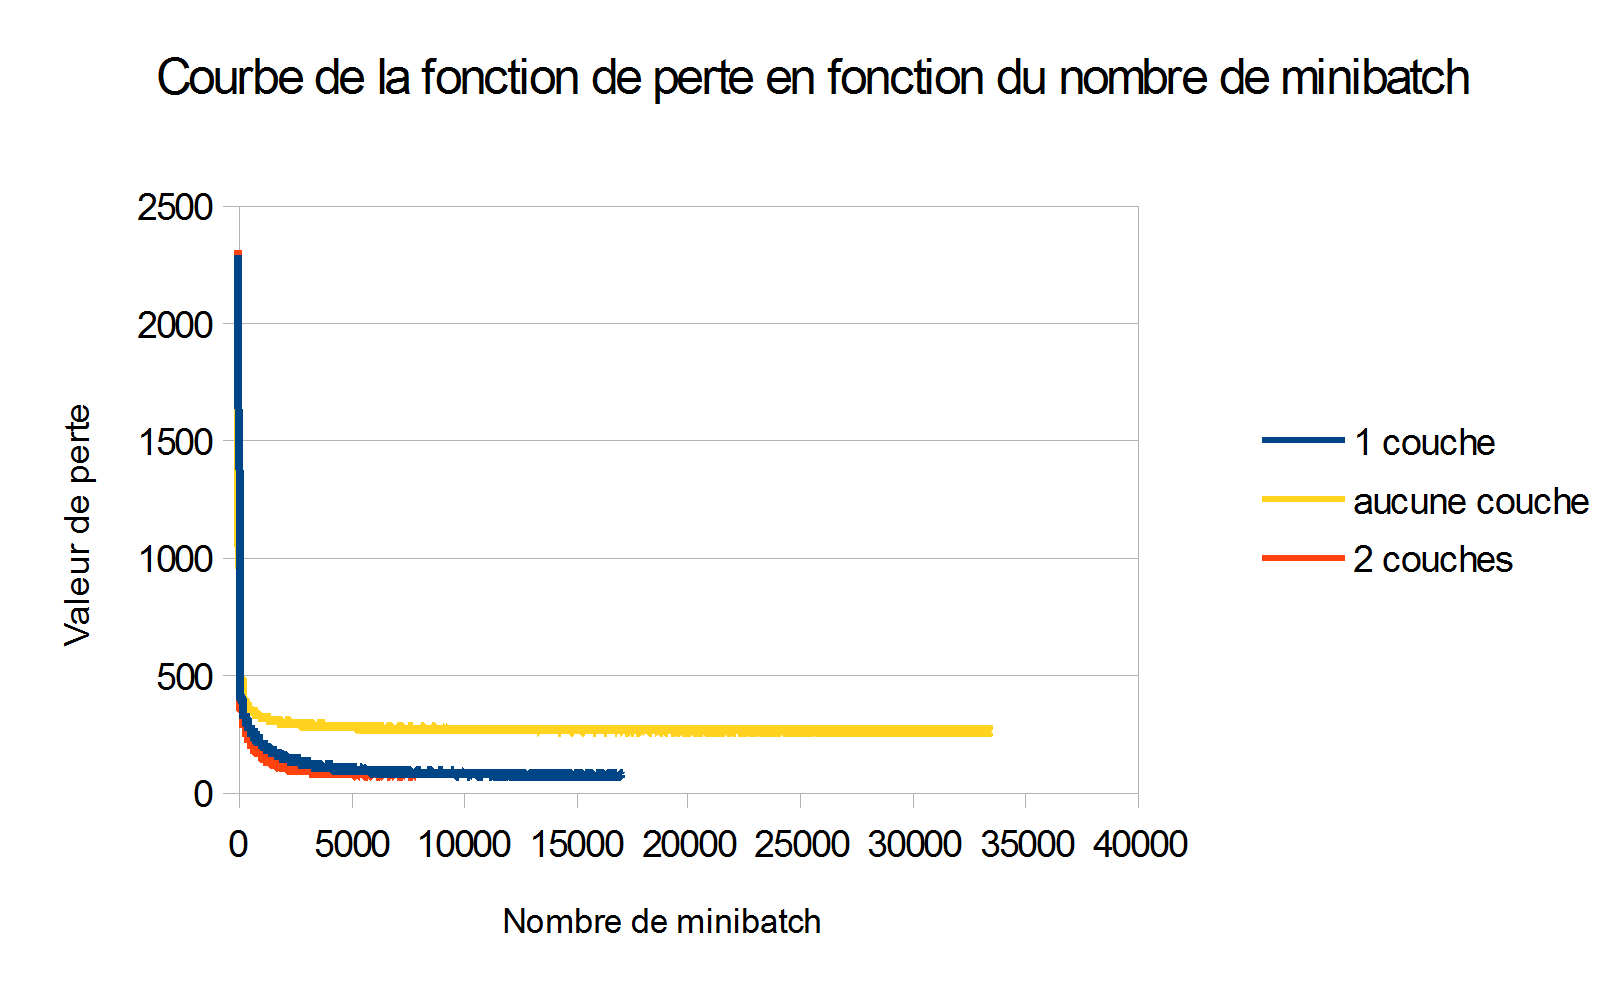
\includegraphics[width=\textwidth,height=\textheight,keepaspectratio]{loss_function.png}
\end{figure}
\begin{figure}[H]
    \label{precision}
    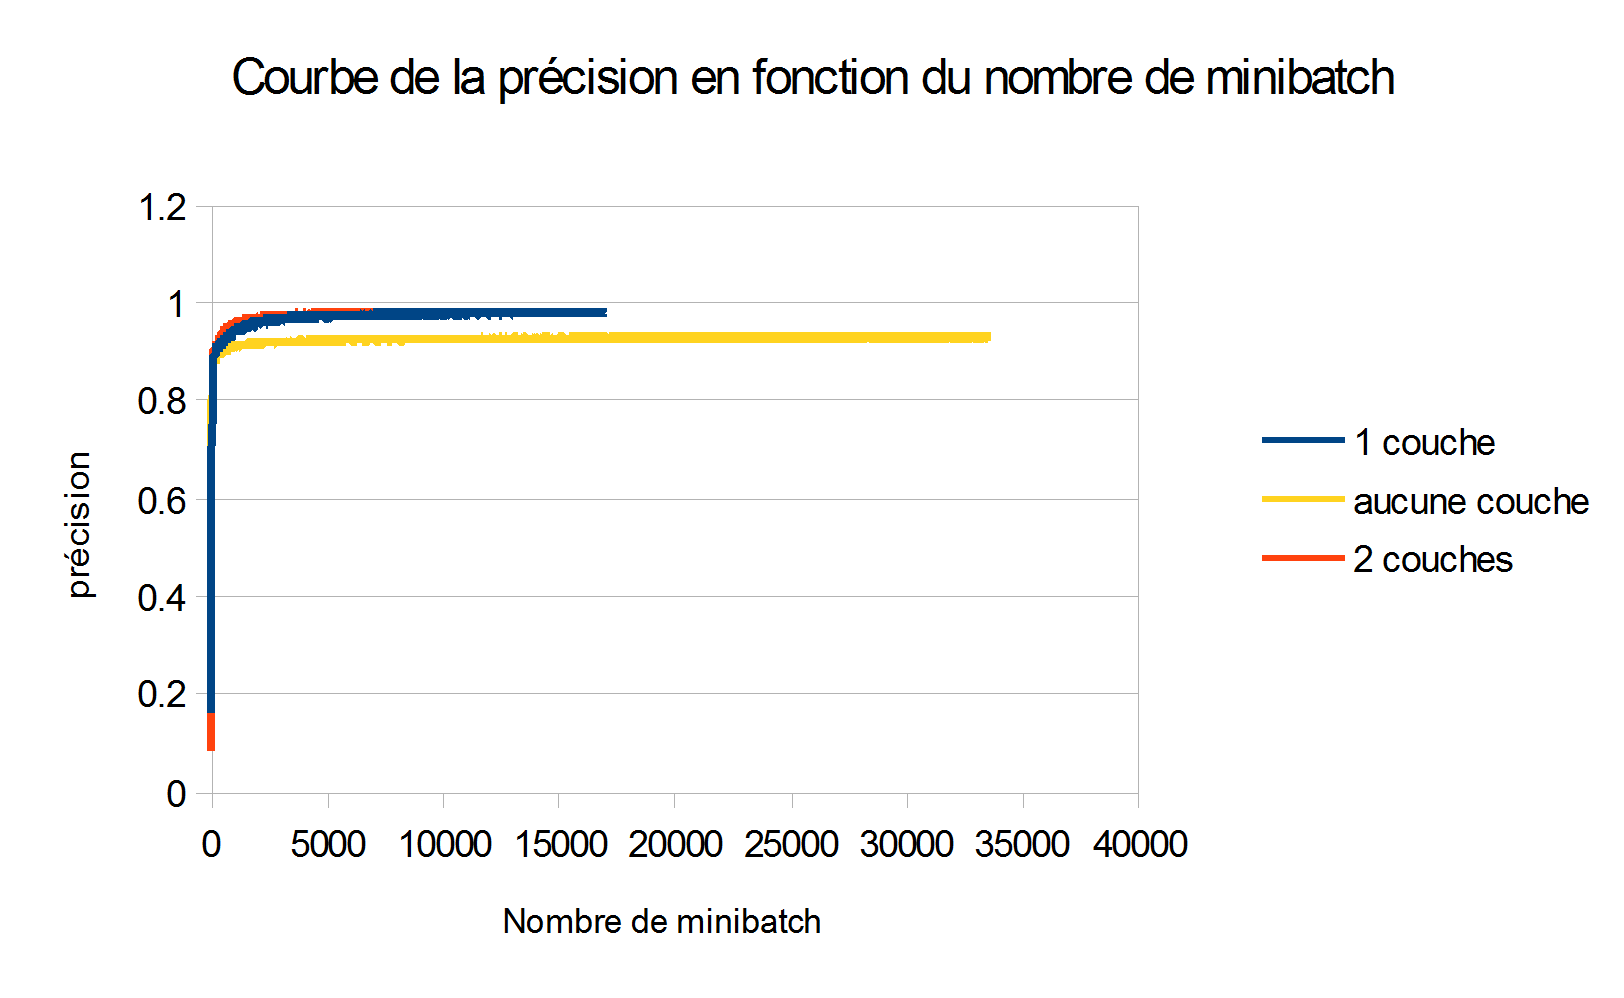
\includegraphics[width=\textwidth,height=\textheight,keepaspectratio]{precision.png}
\end{figure}

Il est possible de voir dans les figures que la performance du réseau à deux couches est très similaire à celle du réseau à une seule couche. Elle a toutefois nécessité beaucoup moins de mini-batch pour atteindre son optimum. Le réseau sans couche cachée est clairement moins performant les deux autres. 
\end{document}
\grid
\grid
